% Versión explicada, sin jerga: una idea por diapositiva, dibujo grande, poco texto.
% Para el director y el jurado. La versión técnica completa está en workflow_lsc.tex.
% Compilar:  latexmk -pdf explicacion_simple.tex
\documentclass[aspectratio=169,11pt]{beamer}
\usepackage[utf8]{inputenc}
\usepackage[T1]{fontenc}
\usepackage[spanish,es-nodecimaldot,es-noshorthands]{babel}
\usepackage[sfdefault,lining]{FiraSans}
\usepackage{icomma}
\usepackage{graphicx}
\usepackage{adjustbox}
\usepackage{tikz}
\usetikzlibrary{arrows.meta,positioning,calc,shapes.geometric,decorations.pathreplacing}

\definecolor{azul}{HTML}{1F4E79}
\definecolor{azulc}{HTML}{DCE8F5}
\definecolor{naranja}{HTML}{D9642B}
\definecolor{naranjac}{HTML}{FBE3D6}
\definecolor{verde}{HTML}{2E7D4F}
\definecolor{verdec}{HTML}{DDF0E4}
\definecolor{gris}{HTML}{6B7280}
\definecolor{grisc}{HTML}{EEF0F3}

\setbeamertemplate{navigation symbols}{}
\setbeamercolor{frametitle}{fg=azul}
\setbeamercolor{normal text}{fg=black!85}
\setbeamerfont{frametitle}{size=\Large,series=\bfseries}
\setbeamertemplate{frametitle}{\vspace{0.25cm}\hspace{0.1cm}\insertframetitle\par\vspace{0.05cm}}
\setbeamertemplate{footline}{\hfill{\scriptsize\color{gris}\insertframenumber}\hspace{0.4cm}\vspace{0.25cm}}
\setbeamersize{text margin left=0.9cm, text margin right=0.9cm}

\tikzset{
  caja/.style={draw=azul, fill=azulc, rounded corners=6pt, line width=1pt, align=center,
               minimum height=1.9cm, text width=2.3cm, font=\large},
  flecha/.style={-{Stealth[length=3.5mm]}, line width=1.6pt, color=gris},
  num/.style={circle, fill=naranja, text=white, font=\bfseries, inner sep=2pt, minimum size=0.62cm},
}
% Texto grande de apoyo al pie de la diapositiva
\newcommand{\persona}[3]{% x, y, escala
      \begin{scope}[shift={(#1,#2)}, scale=#3]
        \draw[line width=1.2pt, color=gris] (0,1.6) circle (0.28);
        \draw[line width=1.2pt, color=gris] (-0.6,1.1) -- (0.6,1.1);
        \draw[line width=1.2pt, color=gris] (0,1.1) -- (0,0);
        \draw[line width=1.2pt, color=azul] (-0.6,1.1) -- (-0.8,0.5) -- (-0.4,0.9);
        \draw[line width=1.2pt, color=azul] (0.6,1.1) -- (0.9,1.7);
        \fill[naranja] (0,1.1) circle (2.5pt);
      \end{scope}}
\newcommand{\idea}[1]{\vfill\begin{center}\large #1\end{center}\vspace{0.2cm}}

\title{\textbf{De la seña a la voz}}
\subtitle{Cómo el prototipo reconoce la Lengua de Señas Colombiana}
\author{Joshua Emmanuel Méndez Ospina\\[2pt]\small Director: Felipe Palta}
\date{\small Pontificia Universidad Javeriana Cali · 30 de septiembre de 2026}

\begin{document}

% ------------------------------------------------------------------ 1
\begin{frame}[plain]
  \vspace{1.2cm}
  {\color{azul}\fontsize{34}{40}\selectfont\bfseries De la seña a la voz\par}
  \vspace{0.3cm}
  {\Large Cómo el prototipo reconoce la Lengua de Señas Colombiana\par}
  \vspace{1.2cm}
  {\large Joshua Emmanuel Méndez Ospina\par}
  {\color{gris}Director: Felipe Palta · Javeriana Cali · 30 de septiembre de 2026\par}
\end{frame}

% ------------------------------------------------------------------ 2
\begin{frame}{Qué hace el sistema}
  \vspace{0.6cm}
  \begin{center}
  \begin{adjustbox}{max width=\linewidth, max totalheight=0.52\textheight}\begin{tikzpicture}[node distance=1.3cm]
    \node[caja, text width=3.0cm] (p) {Una persona\\ hace una seña};
    \node[caja, text width=3.0cm, right=of p] (c) {La cámara\\ la graba};
    \node[caja, text width=3.0cm, right=of c] (m) {El computador\\ la reconoce};
    \node[caja, text width=3.0cm, right=of m, draw=naranja, fill=naranjac] (v) {Y la dice\\ en voz alta:\\ \textbf{«Hola»}};
    \draw[flecha] (p) -- (c); \draw[flecha] (c) -- (m); \draw[flecha] (m) -- (v);
  \end{tikzpicture}\end{adjustbox}
  \end{center}
  \idea{Reconoce \textbf{50 señas} de la LSC (saludos, familia, preguntas, emociones\ldots)\\ y las pronuncia en español. Funciona en un computador normal, sin internet.}
\end{frame}

% ------------------------------------------------------------------ 3
\begin{frame}{El camino completo, en 5 pasos}
  \vspace{0.5cm}
  \begin{center}
  \begin{adjustbox}{max width=\linewidth, max totalheight=0.52\textheight}\begin{tikzpicture}[node distance=0.75cm]
    \node[caja] (a) {Grabar\\ el video};
    \node[caja, right=of a] (b) {Encontrar\\ las manos};
    \node[caja, right=of b] (c) {Ordenar\\ los datos};
    \node[caja, right=of c, draw=naranja, fill=naranjac] (d) {Reconocer\\ la seña};
    \node[caja, right=of d] (e) {Decirla\\ en voz alta};
    \foreach \n/\k in {a/1,b/2,c/3,d/4,e/5} \node[num] at (\n.north west) {\k};
    \draw[flecha] (a) -- (b); \draw[flecha] (b) -- (c); \draw[flecha] (c) -- (d); \draw[flecha] (d) -- (e);
    \node[below=0.25cm of b, color=gris] {MediaPipe};
    \node[below=0.25cm of d, color=gris] {red neuronal};
    \draw[decorate, color=gris, line width=1pt] ($(a.south west)+(0,-0.9)$) -- ($(c.south east)+(0,-0.9)$)
      node[midway, below=2pt, font=\large, color=black!80] {convierten el video en \textbf{números}};
    \draw[color=naranja, line width=1pt] ($(d.south west)+(0,-0.9)$) -- ($(d.south east)+(0,-0.9)$)
      node[midway, below=2pt, font=\large, color=black!80, align=center] {interpreta\\ los números};
  \end{tikzpicture}\end{adjustbox}
  \end{center}
  \idea{En las siguientes diapositivas se explica cada paso.}
\end{frame}

% ------------------------------------------------------------------ 4
\begin{frame}{Los datos: 997 videos de 5 personas}
  \vspace{0.5cm}
  \begin{center}
  \begin{adjustbox}{max width=\linewidth, max totalheight=0.52\textheight}\begin{tikzpicture}[node distance=0.55cm, every node/.style={font=\Large}]
    \node[caja, text width=2.4cm] (s) {\textbf{50}\\ señas};
    \node[right=of s] (x1) {$\times$};
    \node[caja, text width=2.4cm, right=of x1] (p) {\textbf{5}\\ personas};
    \node[right=of p] (x2) {$\times$};
    \node[caja, text width=2.4cm, right=of x2] (r) {\textbf{4}\\ veces cada una};
    \node[right=of r] (ig) {$=$};
    \node[caja, text width=2.4cm, right=of ig, draw=naranja, fill=naranjac] (t) {\textbf{1.000}\\ videos};
  \end{tikzpicture}\end{adjustbox}
  \end{center}
  \vspace{0.3cm}
  \begin{itemize}\large
    \item Cada video es \textbf{una persona haciendo una sola seña}.
    \item Al revisarlos encontramos \textbf{3 videos repetidos} (error del corpus, no de la descarga) $\rightarrow$ quedan \textbf{997}.
    \item Cada seña tiene \textbf{20 videos} (tres tienen 19): las 50 clases están \textbf{balanceadas}.
  \end{itemize}
  \vfill{\small\color{gris} Corpus público LSC50, Universidad de los Andes (2024).}
\end{frame}

% ------------------------------------------------------------------ 5
\begin{frame}{Paso 2: el computador no mira la imagen, mira puntos}
  \begin{center}
    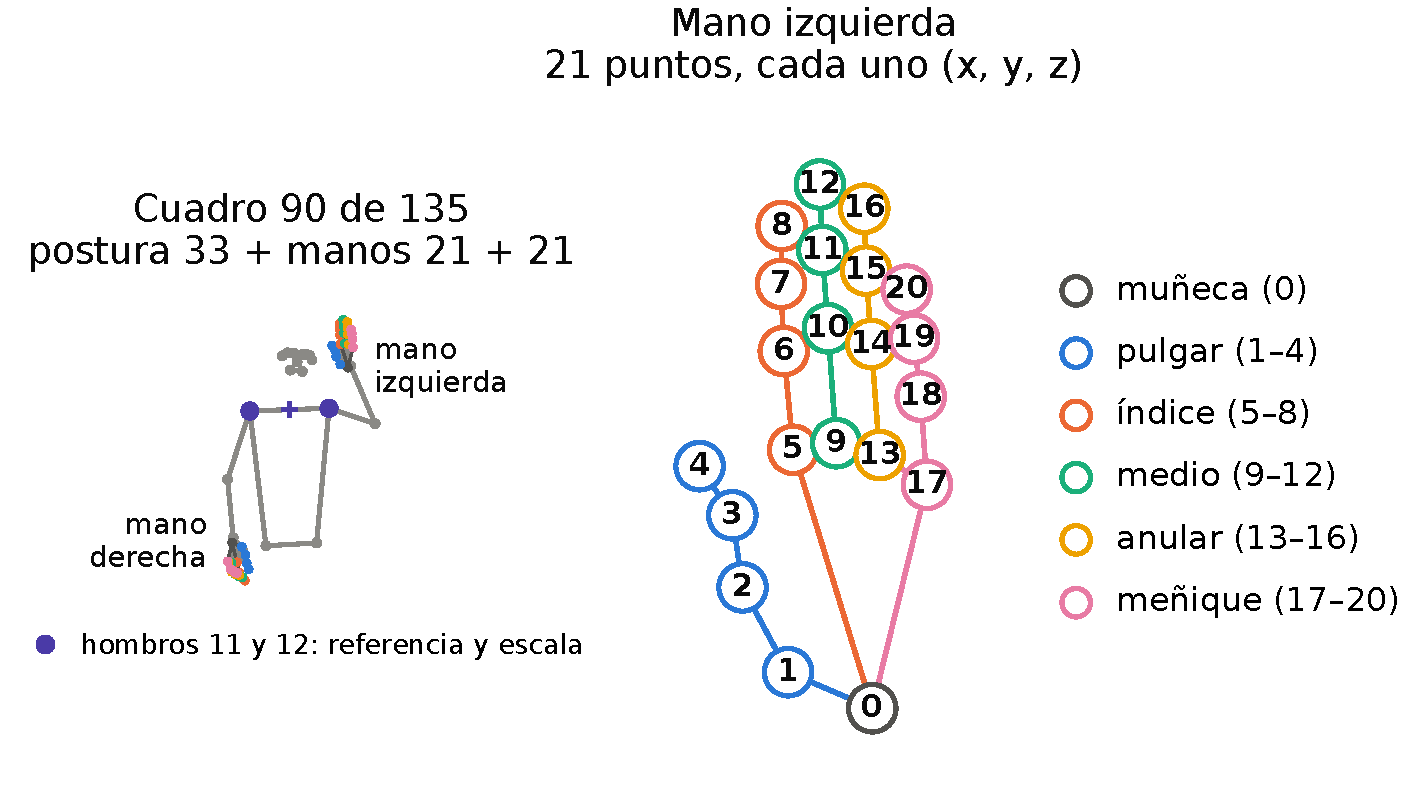
\includegraphics[height=0.6\textheight]{figuras/escritorio_a_esqueleto_0030_0000_0000.pdf}
  \end{center}
  \vspace{-0.2cm}
  \begin{itemize}\large
    \item MediaPipe (una herramienta de Google) encuentra \textbf{21 puntos en cada mano}: la muñeca y 4 por dedo.
    \item Cada punto son \textbf{3 números} (horizontal, vertical y profundidad): {\color{naranja}\textbf{una mano = 21 × 3 = 63 números}}.
  \end{itemize}
\end{frame}

% ------------------------------------------------------------------ 6
\begin{frame}{Paso 2: se hace en todos los cuadros del video}
  \vspace{0.4cm}
  \begin{center}
  \begin{adjustbox}{max width=\linewidth, max totalheight=0.52\textheight}\begin{tikzpicture}
    % película
    \foreach \i in {0,...,7} {
      \draw[fill=grisc, draw=gris] (\i*0.9,0) rectangle ++(0.75,0.9);
      \draw[color=azul, line width=0.8pt] (\i*0.9+0.37,0.2) -- ++(0.05*\i-0.15,0.5);
      \fill[naranja] (\i*0.9+0.37+0.05*\i-0.15,0.7) circle (2pt);
    }
    \node[font=\Large] at (7.9,0.45) {$\cdots$};
    \node[font=\large, below] at (3.5,-0.1) {video de «hola»: \textbf{135 cuadros} (5,6 segundos)};
    \draw[flecha] (8.7,0.45) -- (10.0,0.45) node[midway, above, font=\normalsize, color=gris] {MediaPipe};
    % tabla
    \foreach \j in {0,...,5} \draw[draw=azul, fill=azulc] (10.2, 1.1-\j*0.33) rectangle ++(3.4,0.28);
    \node[font=\large] at (11.9,-1.15) {$\vdots$};
    \node[font=\large, right] at (13.7,0.3) {\textbf{135 filas}};
    \node[font=\normalsize, color=gris] at (11.9,1.65) {una fila por cuadro};
  \end{tikzpicture}\end{adjustbox}
  \end{center}
  \vspace{0.3cm}
  \begin{itemize}\large
    \item Los videos van a \textbf{24 cuadros por segundo}. No se salta ninguno.
    \item Lo importante: \textbf{una muestra es el video completo}, no cada cuadro.\\
          El modelo aprende de 997 muestras, una por seña grabada.
  \end{itemize}
\end{frame}

% ------------------------------------------------------------------ 7
\begin{frame}{Paso 3: no importa dónde esté la persona}
  \vspace{0.3cm}
  \begin{center}
  \begin{adjustbox}{max width=\linewidth, max totalheight=0.52\textheight}\begin{tikzpicture}

    \draw[draw=gris] (0,0) rectangle (5,3.2);
    \persona{1.2}{0.4}{0.8}
    \persona{3.8}{1.0}{1.25}
    \node[font=\large, below, align=center] at (2.5,0) {dos personas en lugares\\ y tamaños distintos};
    \draw[flecha] (5.5,1.6) -- (7.3,1.6);
    \draw[draw=gris] (7.8,0) rectangle (12.8,3.2);
    \persona{10.3}{0.2}{1.4}
    \node[font=\large, below, align=center] at (10.3,0) {medidas desde el centro\\ de los hombros};
    \node[font=\normalsize, color=naranja] at (11.3,1.95) {centro};
  \end{tikzpicture}\end{adjustbox}
  \end{center}
  \idea{Todas las posiciones se miden \textbf{desde el centro de los hombros} y en «anchos de hombros».\\ Así da igual si la persona está más cerca, más lejos o más a un lado.}
\end{frame}

% ------------------------------------------------------------------ 8
\begin{frame}{Paso 3: todas las señas quedan del mismo largo}
  \vspace{0.3cm}
  \begin{center}
  \begin{adjustbox}{max width=\linewidth, max totalheight=0.52\textheight}\begin{tikzpicture}
    % seña larga
    \node[anchor=east, font=\large] at (-0.2,1.6) {«hola», 135 cuadros};
    \foreach \i in {0,...,134} \fill[azul!55] (\i*0.07,1.4) rectangle ++(0.045,0.4);
    % seña corta
    \node[anchor=east, font=\large] at (-0.2,0.2) {«hola», 69 cuadros};
    \foreach \i in {0,...,68} \fill[azul!55] (\i*0.137,0) rectangle ++(0.09,0.4);
    % 30 pasos
    \foreach \i in {0,...,29} {
      \fill[naranja] (\i*0.3238+0.02,-1.35) circle (3pt);
    }
    \node[anchor=east, font=\large, color=naranja] at (-0.2,-1.35) {\textbf{siempre 30 pasos}};
    \draw[flecha] (4.7,-0.2) -- (4.7,-1.05);
  \end{tikzpicture}\end{adjustbox}
  \end{center}
  \vspace{0.2cm}
  \begin{itemize}\large
    \item Se toman \textbf{30 momentos repartidos} del inicio al final de la seña.
    \item Si un momento cae entre dos cuadros, se calcula el punto intermedio (\textbf{interpolación lineal}).
    \item Es como estirar o encoger un dibujo: cambia el largo, \textbf{no la forma} de la seña.
  \end{itemize}
\end{frame}

% ------------------------------------------------------------------ 9
\begin{frame}{Lo que recibe la red: una tabla de 30 × 252 números}
  \vspace{0.3cm}
  \begin{center}
  \begin{adjustbox}{max width=\linewidth, max totalheight=0.52\textheight}\begin{tikzpicture}
    \foreach \x/\w/\c/\t in {0/3.1/azulc/{mano izquierda\\ 63},3.2/3.1/azulc/{mano derecha\\ 63},
                              6.4/3.1/naranjac/{cuánto se movió\\ la izquierda: 63},9.6/3.1/naranjac/{cuánto se movió\\ la derecha: 63}}
      \node[draw=gris, fill=\c, minimum width=\w cm, minimum height=1.1cm, anchor=west, align=center, font=\normalsize] at (\x,0) {\t};
    \draw[decorate, decoration={brace, amplitude=6pt}, line width=1pt] (0,0.75) -- (6.3,0.75)
      node[midway, above=7pt, font=\large] {\textbf{posición}: 126};
    \draw[decorate, decoration={brace, amplitude=6pt}, line width=1pt] (6.4,0.75) -- (12.7,0.75)
      node[midway, above=7pt, font=\large] {\textbf{velocidad}: 126};
    \node[font=\Large, anchor=west] at (13.0,0) {$= \mathbf{252}$};
    \node[font=\normalsize, color=gris, anchor=east] at (-0.1,0) {1 paso};
  \end{tikzpicture}\end{adjustbox}
  \end{center}
  \vspace{0.4cm}
  \begin{itemize}\large
    \item \textbf{Posición}: dónde está cada uno de los 42 puntos de las manos (21 + 21) × 3 números.
    \item \textbf{Velocidad}: cuánto se movió cada punto desde el paso anterior.
    \item Y eso en cada uno de los \textbf{30 pasos} $\rightarrow$ 30 × 252 = \textbf{7.560 números} por seña.
  \end{itemize}
\end{frame}

% ------------------------------------------------------------------ 10
\begin{frame}{Paso 4: la red neuronal lee la seña en orden}
  \vspace{0.3cm}
  \begin{center}
  \begin{adjustbox}{max width=\linewidth, max totalheight=0.52\textheight}\begin{tikzpicture}[node distance=0.6cm]
    \node[caja, text width=2.4cm, fill=grisc, draw=gris] (e) {la tabla\\ 30 × 252};
    \node[caja, text width=2.9cm, right=of e] (c) {\textbf{1.} Detecta\\ movimientos\\ cortos};
    \node[caja, text width=2.9cm, right=of c] (l) {\textbf{2.} Recuerda\\ el orden\\ (ida y vuelta)};
    \node[caja, text width=2.9cm, right=of l] (a) {\textbf{3.} Se fija en\\ los momentos\\ clave};
    \node[caja, text width=2.4cm, right=of a, draw=naranja, fill=naranjac] (s) {50\\ probabili-\\ dades};
    \draw[flecha] (e) -- (c); \draw[flecha] (c) -- (l); \draw[flecha] (l) -- (a); \draw[flecha] (a) -- (s);
    \node[below=0.2cm of c, color=gris] {Conv1D};
    \node[below=0.2cm of l, color=gris, align=center] {LSTM\\ bidireccional};
    \node[below=0.2cm of a, color=gris] {atención};
  \end{tikzpicture}\end{adjustbox}
  \end{center}
  \vspace{0.2cm}
  \begin{itemize}\large
    \item Sí, \textbf{es una LSTM}: la parte que recuerda qué pasó antes y qué viene después.
    \item Una seña no es una foto, es un movimiento: por eso la red lee los 30 pasos \textbf{en orden}.
    \item Construida con \textbf{TensorFlow / Keras}.
  \end{itemize}
\end{frame}

% ------------------------------------------------------------------ 11
\begin{frame}{Cómo aprende la red: con ejemplos que ya tienen nombre}
  \begin{columns}[c]
  \begin{column}{0.5\textwidth}
  \begin{center}
  \begin{adjustbox}{max width=\linewidth, max totalheight=0.52\textheight}\begin{tikzpicture}[node distance=0.45cm, every node/.style={font=\large}]
    \node[caja, text width=3.4cm, minimum height=1cm] (m) {Se le muestra una seña};
    \node[caja, text width=3.4cm, minimum height=1cm, below=of m] (g) {Adivina cuál es};
    \node[caja, text width=3.4cm, minimum height=1cm, below=of g] (e) {Se mide su error};
    \node[caja, text width=3.4cm, minimum height=1cm, below=of e, draw=naranja, fill=naranjac] (a) {Se corrige un poco};
    \draw[flecha] (m) -- (g); \draw[flecha] (g) -- (e); \draw[flecha] (e) -- (a);
    \draw[flecha] (a.east) -- ++(0.7,0) |- (m.east);
    \node[font=\normalsize, color=gris, align=center] at (3.3,-2.0) {se repite\\ miles de\\ veces};
  \end{tikzpicture}\end{adjustbox}
  \end{center}
  \end{column}
  \begin{column}{0.48\textwidth}\large
    Los videos se separan en tres grupos:

    \vspace{0.3cm}
    \colorbox{azulc}{\textbf{Aprender}} la red practica con ellos.

    \vspace{0.2cm}
    \colorbox{grisc}{\textbf{Ajustar}} sirven para saber cuándo parar (2 por seña).

    \vspace{0.2cm}
    \colorbox{naranjac}{\textbf{Examen final}} la red \textbf{nunca} los vio; de aquí salen los resultados.

    \vspace{0.3cm}
    Lo que se entrena es la red. MediaPipe se usa tal cual.
  \end{column}
  \end{columns}
\end{frame}

% ------------------------------------------------------------------ 12
\begin{frame}{Paso 5: decide y habla}
  \vspace{0.3cm}
  \begin{center}
  \begin{adjustbox}{max width=\linewidth, max totalheight=0.52\textheight}\begin{tikzpicture}
    \foreach \y/\g/\p/\w/\col in {2/hola/90\,\%/9.02/naranja, 1.2/¿por qué?/{0,9\,\%}/0.089/gris!60, 0.4/niño/{0,5\,\%}/0.051/gris!60} {
      \node[anchor=east, font=\large] at (-0.2,\y) {\g};
      \fill[\col] (0,\y-0.25) rectangle ++(\w,0.5);
      \node[anchor=west, font=\large] at (\w+0.15,\y) {\p};
    }
    \draw[dashed, line width=1.2pt, color=verde] (1.8,-0.2) -- (1.8,2.6) node[above, font=\large] {umbral 20\,\%};
    \node[anchor=west, font=\large, color=gris] at (0,-0.55) {\ldots y las otras 47 señas, con menos};
  \end{tikzpicture}\end{adjustbox}
  \end{center}
  \begin{itemize}\large
    \item La red da una probabilidad para \textbf{cada una de las 50 señas}.
    \item Si la más alta supera el umbral, el sistema \textbf{la dice en voz alta}: «Hola».
    \item Si no, no dice nada y \textbf{pide repetir} la seña.
  \end{itemize}
\end{frame}

% ------------------------------------------------------------------ 13
\begin{frame}{¿Qué tan bien funciona?}
  \vspace{0.6cm}
  \begin{columns}[t]
  \begin{column}{0.47\textwidth}
    \begin{center}
      {\color{gris}\Large Con personas que ya conocía}\\[0.3cm]
      {\color{azul}\fontsize{60}{64}\selectfont\bfseries 88\,\%}\\[0.3cm]
      \large acierta a la primera
    \end{center}
  \end{column}
  \begin{column}{0.47\textwidth}
    \begin{center}
      {\color{gris}\Large Con personas nuevas}\\[0.3cm]
      {\color{naranja}\fontsize{60}{64}\selectfont\bfseries 58\,\%}\\[0.3cm]
      \large acierta a la primera\\ \textbf{77\,\%} si cuenta sus 3 primeras opciones
    \end{center}
  \end{column}
  \end{columns}
  \idea{La cifra que importa es la de \textbf{personas nuevas}:\\ así le iría con alguien real que el sistema nunca vio.}
\end{frame}

% ------------------------------------------------------------------ 14
\begin{frame}{Cómo se probó con personas nuevas}
  \vspace{0.3cm}
  \begin{center}
  \begin{adjustbox}{max width=\linewidth, max totalheight=0.52\textheight}\begin{tikzpicture}
    \foreach \r in {0,...,4} {
      \node[anchor=east, font=\large] at (-1.1,-\r*0.75) {Ronda \the\numexpr\r+1\relax};
      \foreach \c in {0,...,4} {
        \ifnum\c=\r
          \node[draw=naranja, fill=naranjac, minimum width=2.0cm, minimum height=0.55cm, font=\normalsize] at (\c*2.3,-\r*0.75) {examen};
        \else
          \node[draw=azul, fill=azulc, minimum width=2.0cm, minimum height=0.55cm, font=\normalsize] at (\c*2.3,-\r*0.75) {aprende};
        \fi
      }
    }
    \foreach \c in {0,...,4} \node[font=\normalsize, color=gris] at (\c*2.3,0.65) {persona \the\numexpr\c+1\relax};
    \foreach \r/\v in {0/46,1/53,2/61,3/62,4/69} \node[anchor=west, font=\large] at (10.6,-\r*0.75) {acierta \textbf{\v\,\%}};
  \end{tikzpicture}\end{adjustbox}
  \end{center}
  \idea{En cada ronda se deja \textbf{una persona fuera} del aprendizaje y se usa como examen.\\ El 58\,\% es el promedio de las 5 rondas.}
\end{frame}

% ------------------------------------------------------------------ 15
\begin{frame}{Dónde se equivoca: con señas que se parecen}
  \vspace{0.8cm}
  \begin{center}
  \begin{adjustbox}{max width=\linewidth, max totalheight=0.52\textheight}\begin{tikzpicture}[every node/.style={font=\Large}]
    \node[caja, text width=2.6cm, minimum height=1.1cm] (a1) {niño};
    \node[caja, text width=2.6cm, minimum height=1.1cm, right=1.8cm of a1] (a2) {niña};
    \draw[{Stealth[length=3mm]}-{Stealth[length=3mm]}, line width=1.5pt, color=naranja] (a1) -- (a2);
    \node[caja, text width=2.6cm, minimum height=1.1cm, right=1.3cm of a2] (b1) {¿cómo estás?};
    \node[caja, text width=2.6cm, minimum height=1.1cm, right=1.8cm of b1] (b2) {¿cómo?};
    \draw[{Stealth[length=3mm]}-{Stealth[length=3mm]}, line width=1.5pt, color=naranja] (b1) -- (b2);
  \end{tikzpicture}\end{adjustbox}
  \end{center}
  \vspace{0.3cm}
  \begin{itemize}\large
    \item Estas parejas se confunden \textbf{en los dos sentidos}.
    \item «Más o menos» no se acertó ni una vez: el sistema dice «poco» o «yo».
    \item Los errores no son al azar: salen donde las señas \textbf{se parecen de verdad}.
  \end{itemize}
\end{frame}

% ------------------------------------------------------------------ 16
\begin{frame}{¿Hacía falta una red que lea el orden? Sí}
  \vspace{0.3cm}
  \begin{center}
  \begin{adjustbox}{max width=\linewidth, max totalheight=0.52\textheight}\begin{tikzpicture}
    \foreach \y/\n/\v/\col in {2.4/Nuestra red (lee el orden)/58/naranja, 1.6/Random Forest/42/gris!55, 0.8/SVM/26/gris!55, 0/Perceptrón multicapa/25/gris!55} {
      \node[anchor=east, font=\large] at (-0.2,\y) {\n};
      \pgfmathsetmacro{\w}{\v*0.13}
      \fill[\col] (0,\y-0.27) rectangle (\w,\y+0.27);
      \node[anchor=west, font=\large\bfseries] at (\w+0.15,\y) {\v\,\%};
    }
  \end{tikzpicture}\end{adjustbox}
  \end{center}
  \idea{Los métodos más simples solo ven un resumen de la seña, no su orden.\\ Con personas nuevas aciertan menos, y la diferencia es estadísticamente significativa.}
\end{frame}

% ------------------------------------------------------------------ 17
\begin{frame}{¿Qué tan rápido responde?}
  \vspace{0.8cm}
  \begin{center}
  \begin{adjustbox}{max width=\linewidth, max totalheight=0.52\textheight}\begin{tikzpicture}
    \fill[azulc] (0,0) rectangle (11,1);
    \node[font=\Large] at (5.5,0.5) {la persona hace la seña: \textbf{2,5 segundos}};
    \fill[naranja] (11,0) rectangle (11.6,1);
    \draw[flecha] (12.9,1.5) -- (11.7,0.9);
    \node[anchor=west, font=\Large, align=left] at (13.0,1.6) {el sistema\\ responde en\\ \textbf{0,036 s}};
    \draw[line width=1pt] (0,-0.25) -- (0,-0.45) (11,-0.25) -- (11,-0.45);
    \node[font=\large, color=gris] at (0,-0.75) {tecla};
    \node[font=\large, color=gris] at (11,-0.75) {fin de la ventana};
  \end{tikzpicture}\end{adjustbox}
  \end{center}
  \idea{La máquina tarda \textbf{36 milésimas} en reconocer y ordenar hablar.\\ Casi toda la espera es el tiempo de hacer la seña. Todo corre en un portátil, sin tarjeta gráfica.}
\end{frame}

% ------------------------------------------------------------------ 18
\begin{frame}{Lo que sigue}
  \vspace{0.4cm}
  \begin{itemize}\large
    \setlength\itemsep{0.45cm}
    \item \textbf{Prueba con una persona real}: el profesor de LSC vinculado (LSC, Javeriana) aceptó ayudar.
    \item Esa prueba debe hacerse en \textbf{condiciones parecidas a las del corpus}: a unos 2 m de la cámara, fondo liso y buena luz.
    \item Hay que acordar con el director cómo se hace esa prueba (cuántas repeticiones, cuánto dura) y el umbral de confianza.
  \end{itemize}
  \vfill
  \begin{center}\Large\color{azul}\textbf{¿Preguntas?}\end{center}
  \vspace{0.3cm}
\end{frame}

\end{document}
